\documentclass[conference,compsoc,11pt]{IEEEtran}

\usepackage{multirow}
\usepackage{amsmath}
\usepackage{dsfont}
\usepackage{bm}
\usepackage{booktabs}
\usepackage{graphics}

\usepackage{bookmark}% loads hyperref too
    \hypersetup{
        %pdftitle={Fundamentos de C\'alculo},
        %pdfsubject={C\'alculo diferencial},
        bookmarksnumbered=true,
        bookmarksopen=true,
        bookmarksopenlevel=1,
        hidelinks,% remove border and color
        pdfstartview=Fit, % Fits the page to the window.
        pdfpagemode=UseOutlines, %Determines how the file is opening in Acrobat; the possibilities are UseNone, UseThumbs (show thumbnails), UseOutlines (show bookmarks), FullScreen, UseOC (PDF 1.5), and UseAttachments (PDF 1.6). If no mode if explicitly chosen, but the bookmarks option is set, UseOutlines is used.
    }

\usepackage{siunitx}
    
\usepackage[style=verbose]{biblatex}
\addbibresource{./bibliography.bib}

\usepackage[OT1]{fontenc}
\usepackage{glossaries} % certain packages that must be loaded before glossaries, if they are required: hyperref, babel, polyglossia, inputenc and fontenc
\setacronymstyle{long-short}
\newacronym{hf}{HF}{Heart Failure}
\newacronym{lr}{LR}{Logistic Regression}
\newacronym{rf}{RF}{Random Forest}
\newacronym{roc}{ROC}{Receiver Operating Characteristic}
\newacronym{auc}{AUC}{Area Under Curve}
\newacronym{ifhc}{IFHC}{Increase Force of Heart Contraction}

% *** CITATION PACKAGES ***
%
%\ifCLASSOPTIONcompsoc
%  \usepackage[nocompress]{cite}
%\else
%  \usepackage{cite}
%\fi

% *** GRAPHICS RELATED PACKAGES ***
%
\ifCLASSINFOpdf
\else
\fi

%\hyphenation{op-tical net-works semi-conduc-tor}
\usepackage{graphicx}
\graphicspath{ {../output/} }


\begin{document}

\title{Heart Failure: predicting hospital re-admission after 6 months\\
\large Statistical Learning for Healthcare Data (056867) -- A.Y. 2022/2023\\
Prof. M. Ferrario and Prof. A. M. Paganoni}

\author{
    \IEEEauthorblockN{
        Teo Bucci\IEEEauthorrefmark{1},
        Giulia Montani\IEEEauthorrefmark{1}
        and Alice Traversa\IEEEauthorrefmark{2}}
    \IEEEauthorblockA{
        \IEEEauthorrefmark{1}M.Sc. Mathematical Engineering
        \IEEEauthorrefmark{2}M.Sc. Biomedical Engineering,
        Politecnico di Milano\\
        Email: \{teo.bucci, giulia.montani, alice.traversa\}@mail.polimi.it\\
        Code available at: \href{https://github.com/teobucci/slhd}{\texttt{github.com/teobucci/slhd}}
    }
}

\maketitle

%\begin{abstract}
%\end{abstract}
\IEEEpeerreviewmaketitle

%!TEX root = ../report.tex
\section{Introduction}

\gls{hf} is a prevalent condition with high re-admission rates: the literature\footcite{Bragazzi2021Burden} states that the number of \gls{hf} cases worldwide almost doubled from 33.5 million in 1990 to 64.3 million in 2017.

Studies\footcite{Groenewegen2020Epidemiology} also suggest that half of the patients diagnosed with \gls{hf} will be re-admitted once within a year and 20\% will be re-admitted twice or more. The focus of this analysis is on predicting the re-admission within 6 months for \gls{hf} patients.

However, our emphasis extends beyond prediction performance; we prioritize the development of an interpretable model that healthcare professionals can easily understand. By examining patient characteristics and clinical variables, we aim to identify key predictors and provide valuable insights for targeted interventions and personalized care plans.


%!TEX root = ../report.tex
\section{Materials and methods}\label{sec:materials-methods}

%\footcite{Zhang2021Electronic}
The dataset was collected from \num{2008} patients with heart failure who were admitted to a hospital in Sichuan, China between 2016 and 2019, 773 of which were readmitted within 6 months.

A total of 168 variables were provided, which included basic patient characteristics such as age, sex, height, weight, occupation, admission department, visit times, etc. Clinical characteristics such as respiratory rate, systolic blood pressure, diastolic blood pressure, hemoglobin, red blood cells, D dimer, etc. It also included comorbidities such as diabetes, dementia, liver disease, etc.

Variables are of both types: categorical (binary and multi-class) and numerical (continuous and integer).

The majority of patients had age in the 59-89 range, namely a total of 1675 patients accounting for 86.07\% of the total. Regarding sex, 58.22\% were females and 41.78\% were males.

73.54\% suffered a whole \gls{hf}, while 23.84\% suffered a Left \gls{hf} and 2.62\% a Right \gls{hf}.

The other dataset provided contains drugs information: which drugs each patient took.

The problem is framed as a binary classification problem, one for patients that were readmitted to the hospital within 6 months, and another for those who were not.

\subsection{Data cleaning}\label{sec:data-cleaning}

To begin with, we merged the information of the drugs to the main dataset, but since there were 18 drugs, we grouped them into four categories: Diuretics, Vasodilatory, Inhibitor, \gls{ifhc}.

We removed the 57 dead patients and all information on re-hospitalizations prior to 6 months. We also identified and removed 5 patients with inconsistent information: their \texttt{DestinationDischarge} was \texttt{Died} but their outcome during hospitalization wasn't \texttt{Dead}.

\subsubsection{Missing values}

In healthcare datasets, missing values are a big concern. The first step was to inspect the situation:
\begin{itemize}
    \item among the numerical variables, 105 contained NaNs;
    \item among the categorical variables, 1 contained NaNs, which was \texttt{occupation} 1.34\% of missing, which we imputed with the most frequent.
\end{itemize}

% \autoref{fig:missing-values} shows the percentages of missing values in the numerical variables.

% \begin{figure}[htpb]
%     \centering
%     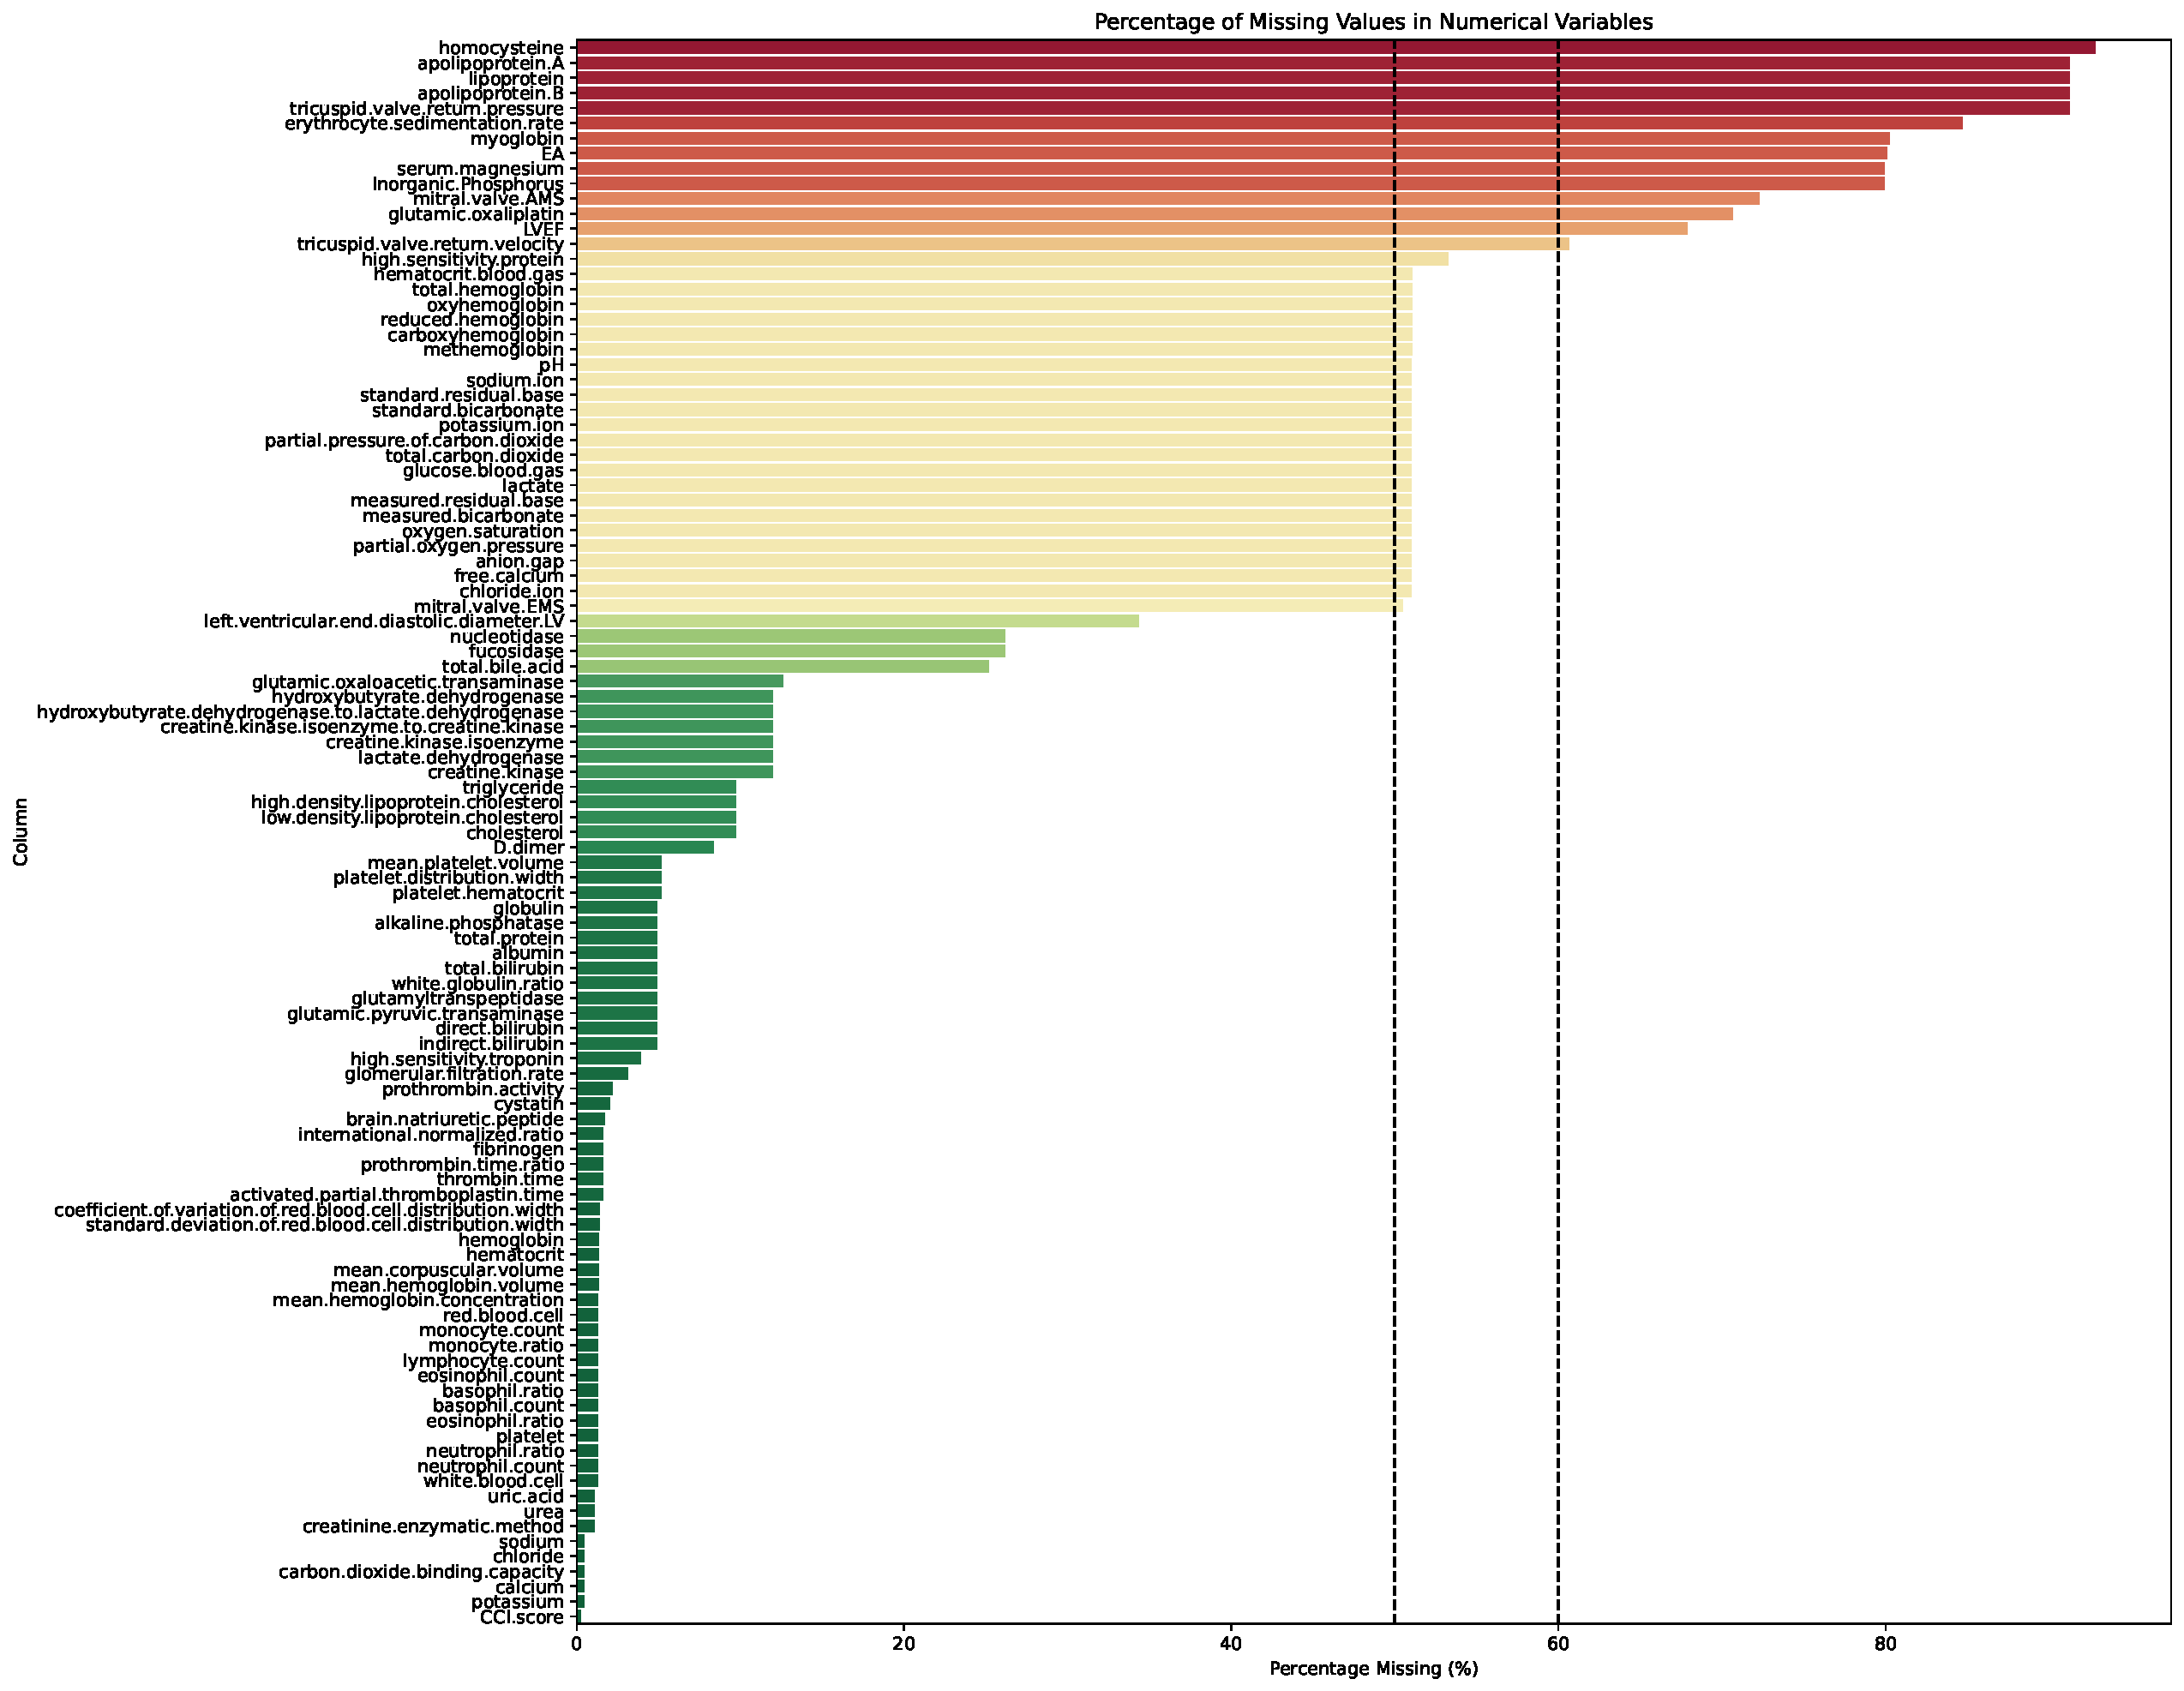
\includegraphics[width=3.1in]{missing_values_percentages.pdf}
%     \caption{Percentage of missing values.}
%     \label{fig:missing-values}
% \end{figure}

All 14 variables with over 60\% missing were discarded, while for those with 50\% to 60\% missing we computed whether there was any variable in the sub-50\% missing part of the dataset with more than 0.80 correlation. If that was the case, we discarded them: 9 variables were removed.

Finally, among the remaining ones in the 50\% to 60\% missing range we computed the correlation matrix, clustered with hierarchical clustering, with the aim of seeing a clearer block structure, see \autoref{fig:clustered-correlation-matrix}. With this techniques we discarded 3 more variables.

\begin{figure}[htpb]
    \centering
    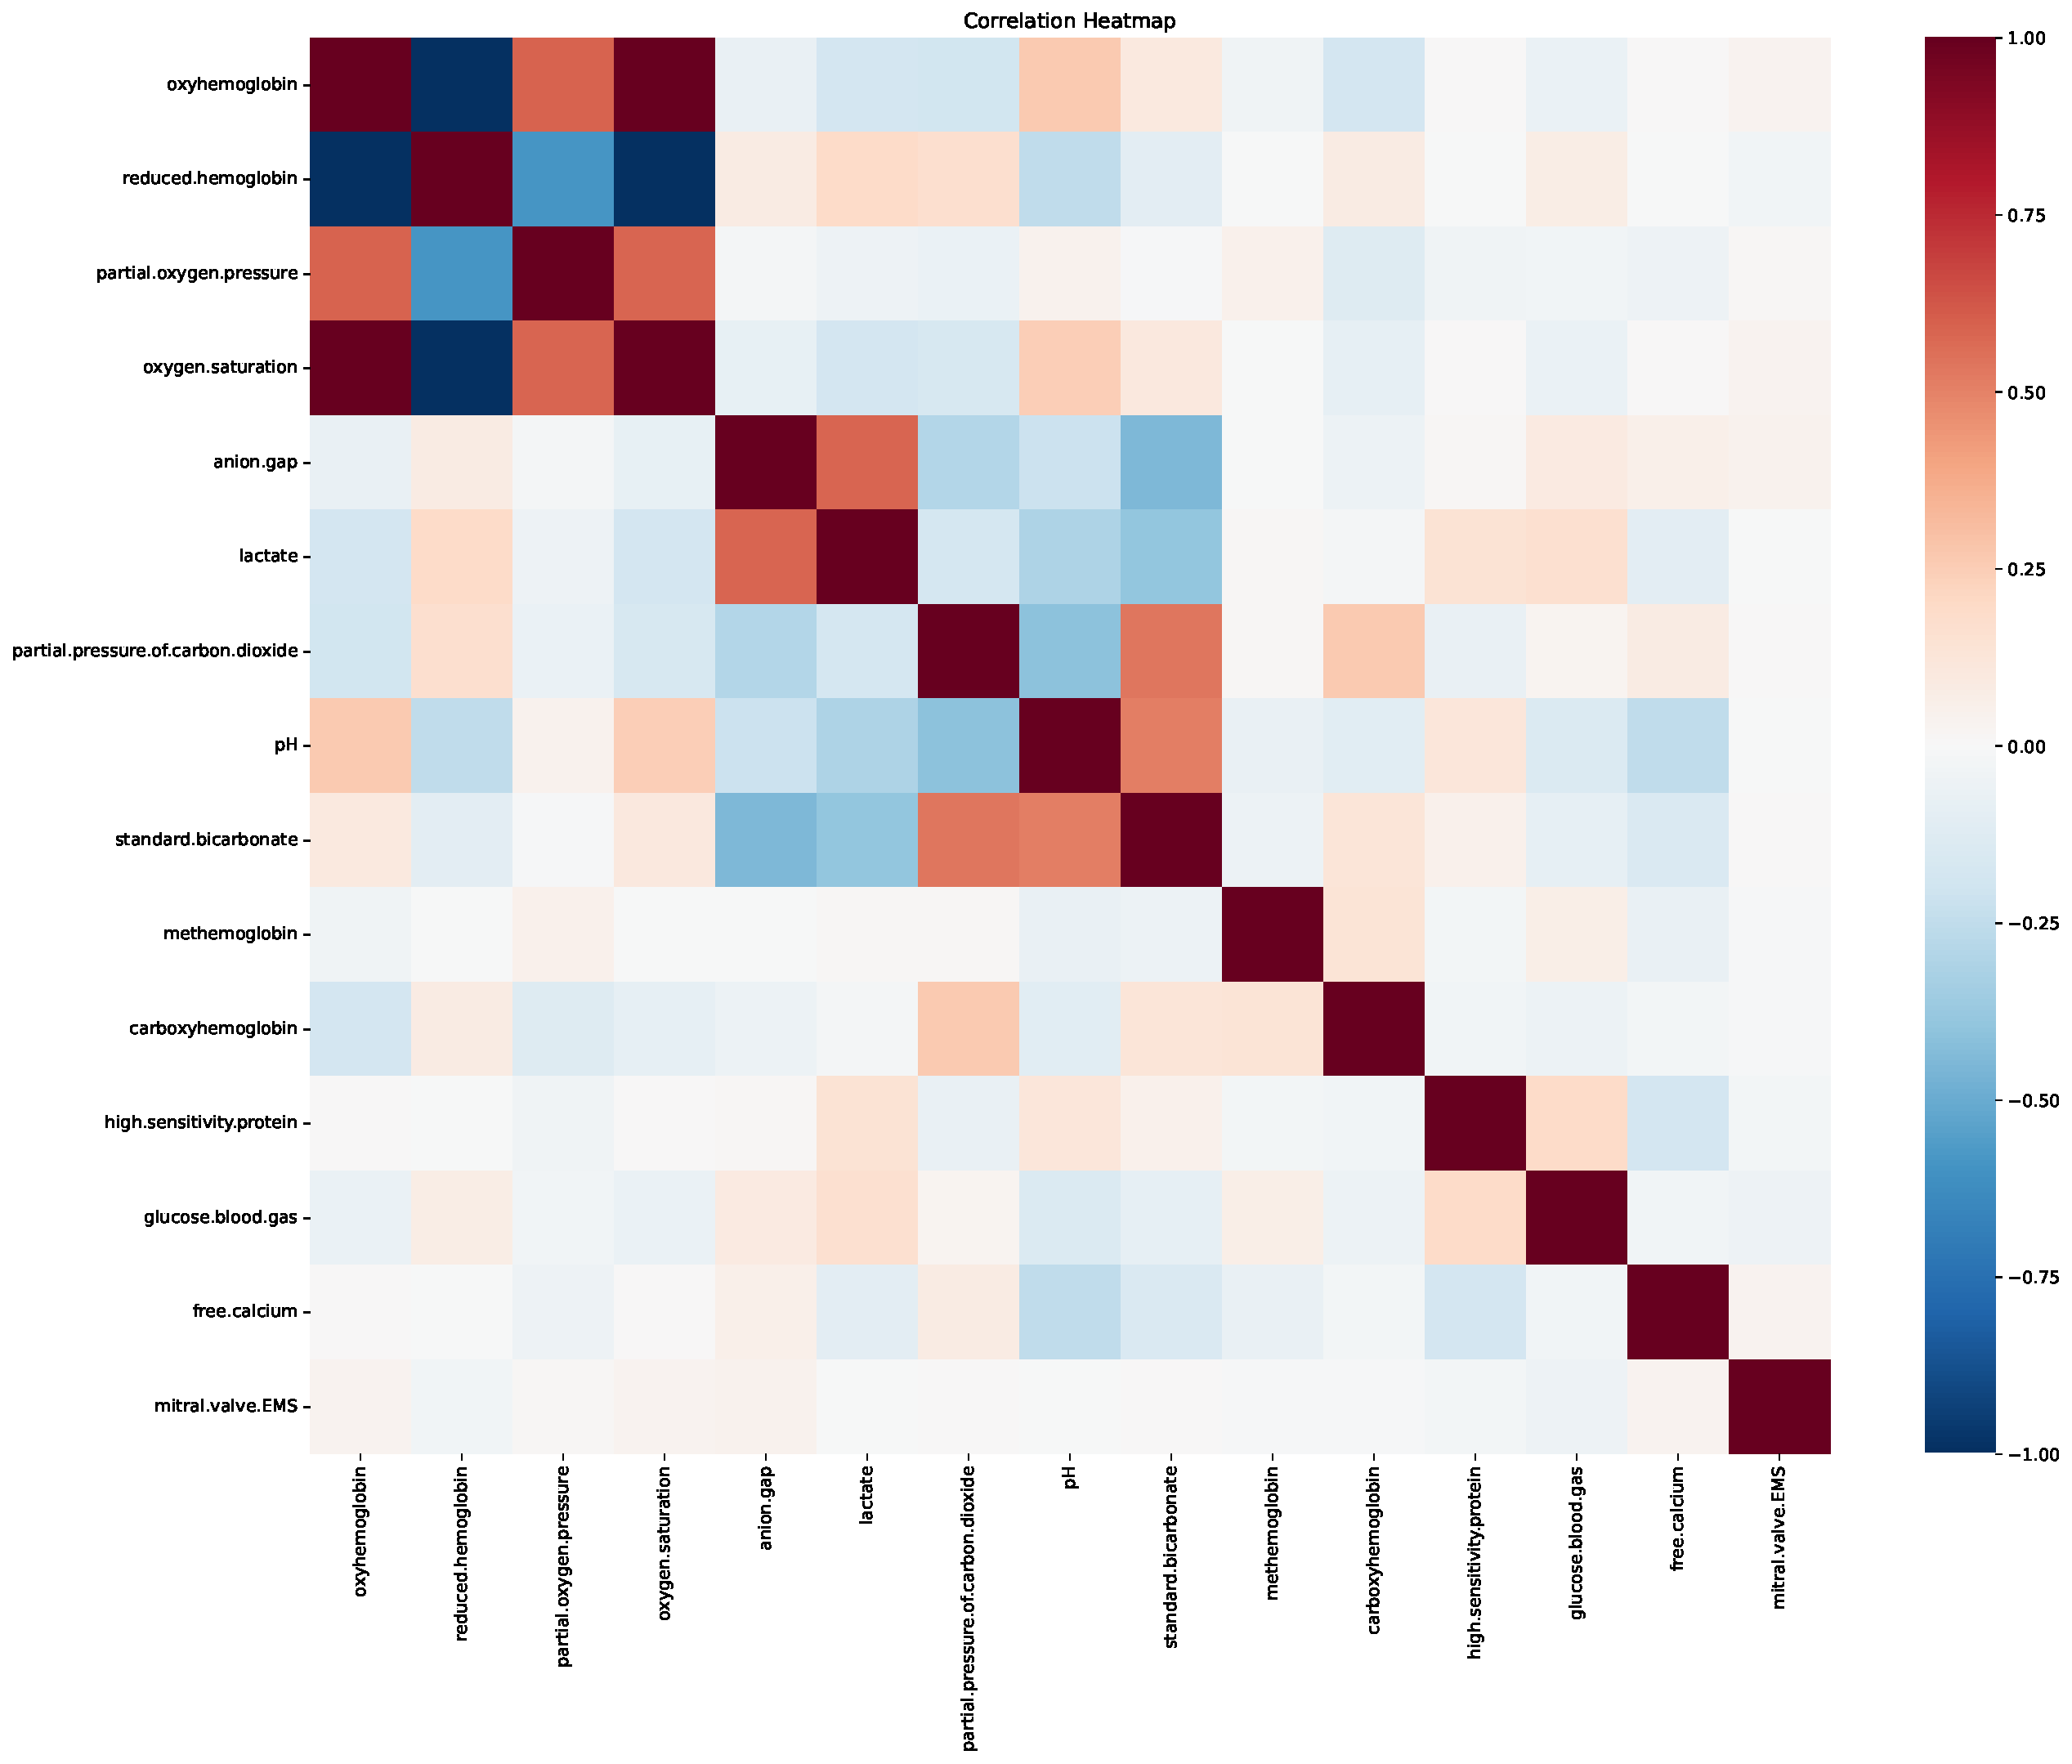
\includegraphics[width=3.1in]{clustered_correlation_matrix.pdf}
    \caption{Correlation matrix of variables with 50\%-60\% missing values.}
    \label{fig:clustered-correlation-matrix}
\end{figure}

\subsubsection{Outlier analysis}\label{sec:outlier-analysis}

An overall histogram of all numerical variables made very clear that there were many outliers in the data.

The approach we followed was to identify them and judge one by one whether or not the values were physiologically possible or not, by checking the literature. In that case, instead of discarding the patient completely, we set the value to NaN to impute it later. During the approach we tried to be as conservative as possible to retain as much information as possible, but simultaneously give to the models high quality data that would enable good separation.

Outliers were identified by calculating the sample $Z$-score of each variable:
\begin{align*}
    Z\text{-score} = \frac{X-\bar{X}}{s}
\end{align*}
where $\bar{X}$ is the sample mean and $s$ is the sample standard deviation.

A threshold of 3 or above was applied to detect them, depending on the specific variable.

After this procedure, there were still three variables that showed possible outliers: \texttt{eosinophil.count}, \texttt{high.sensitivity.troponin} and \texttt{glutamic.pyruvic.transaminase}. However, these variables were marked by many models as important, so we decided to keep them anyway without changes. We suspect there may have been discordances in inserting the values, i.e. for some patients with some unit of measure, for other patients with another unit. We strongly recommend double checking these variables.

\subsubsection{Removing low variance variables}

Among the categorical variables, we removed 16 variables with more than 95\% dominance in values counts, while for the numerical variables we removed 2 constant ones.

\subsubsection{Correlation analysis}

Using clinical knowledge, we inspected some groups of variables we thought could be quite correlated, then we proceeded at discarding variables with more than 0.85 correlation with the others, ultimately removing 12 more variables.

Overall, we were able to discard 62 variables only with preprocessing.

\subsection{Modeling}

The dataset was split according to an 85:15 train-test ratio, preserving the target proportions, and part of the training was designated to validation set.

%All statistical analyses were carried out using Python and mainly the Scikit-learn\footcite{scikit-learn} library.

\subsubsection{Preprocessing categorical data}

Categorical variables were encoded using one-hot encoding.

\subsubsection{Preprocessing numerical data}

Numerical variables were imputed using a KNN imputer with 5 neighbours and then standardized for letting the training converge.

\subsubsection{Class imbalance}

The dataset was a bit imbalanced, with 39.6\% of observations belonging to class 1 (positives). To tackle the problem, whenever the model allowed for it, we passed class weights based on the inverse of percentage of samples over the total.

\subsubsection{Performance indexes}

The main metric used to compare models was the \gls{auc} under the \gls{roc} curve.

\subsection{Feature selection}

Ideally we wanted to perform a backward selection. However, since the initial number of features is 131, the process is very computationally intensive (about 20 seconds per feature to be removed) and greedy, so we would risk discarding important variables too soon. To speed up the process we developed the following method:

\begin{itemize}
    \item Train a \gls{lr} with strong $L^1$ penalty to select a set $S_\text{LR}$ of features.
    \item Train a \gls{rf} and create an $S_\text{RF}$ set of features made by the top 30 features by impurity decrease importance.
    \item Create a set $S_\text{reduced} = S_\text{LR} \cup S_\text{RF}$. The reason for this is that the way \gls{lr} and \gls{rf} select variables is very different, in fact the intersection $S_\text{LR} \cap S_\text{RF}$ was very small. In this way we take advantage of both.
\end{itemize}

We could now perform a backward selection based on this $S_\text{reduced}$ set of features, and inspecting the evolution of the \gls{auc} we selected a suitable number of features $S^\star_1$. Then, since the results are often different, we performed a forward selection from 0 to 10 features on the same model to get the set $S^\star_2$, and finally we took the union of the two as our final features set $S^\star = S^\star_1 \cup S^\star_2$ of 13 variables.

For visualization purposes, in \autoref{fig:distribution-target} we plotted the KDE of some features in $S^\star$ separately with the respect to the target.

It's really clear the difference in distribution of the \texttt{creatinine.enzymatic.method}, we expect it to be important in the final model.

\begin{figure}
    \centering
    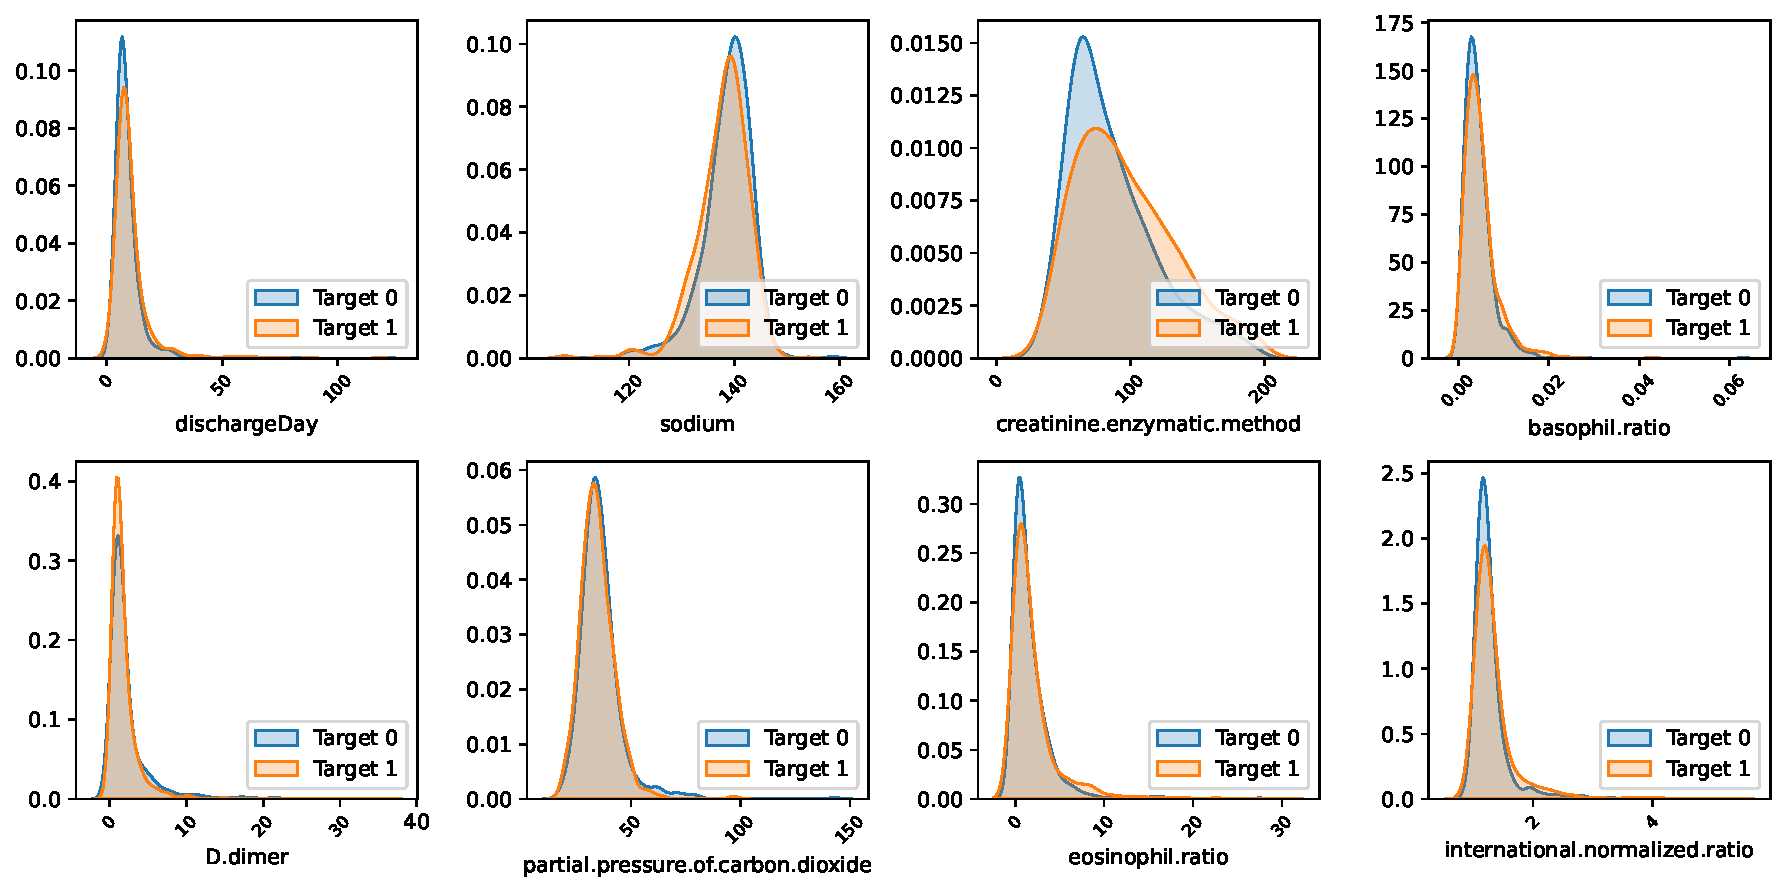
\includegraphics[width=3.1in]{distribution_wrt_target.pdf}
    \caption{Distribution with the respect to the target of sodium and creatinine enzymatic method.}
    \label{fig:distribution-target}
\end{figure}

\subsubsection{Model selection}

We trained 6 different classifiers on the unscaled selected features with a 5-fold stratified cross-validation to tune the hyperparameters.
Besides those, we made an attempt with an SVM, but the training failed to converge except on the scaled data (which makes interpretability harder) and didn't perform well, therefore we don't include it.


%!TEX root = ../report.tex
\section{Results}

\subsection{Model comparison}

\autoref{tab:performance} shows the performance of the different models on the test set after the hyperparameter tuning.
Even though it's not the most performing model, we choose the \gls{lr} for its superior interpretability and simplicity, at the cost of just one percentage point in performance with respect to the \gls{rf}.

\autoref{fig:roc-comparison} shows the \gls{roc} curves of all the models.

\begin{table}
\centering
\caption{Comparison of performance.}
\label{tab:performance}
\begin{tabular}{lr}
\toprule
                 Model &    AUC \\
\midrule
RandomForestClassifier & 0.6769 \\
    LogisticRegression & 0.6702 \\
            GaussianNB & 0.6452 \\
DecisionTreeClassifier & 0.5943 \\
  KNeighborsClassifier & 0.5681 \\
         MLPClassifier & 0.5028 \\
\bottomrule
\end{tabular}
\end{table}


\begin{figure}[htpb]
    \centering
    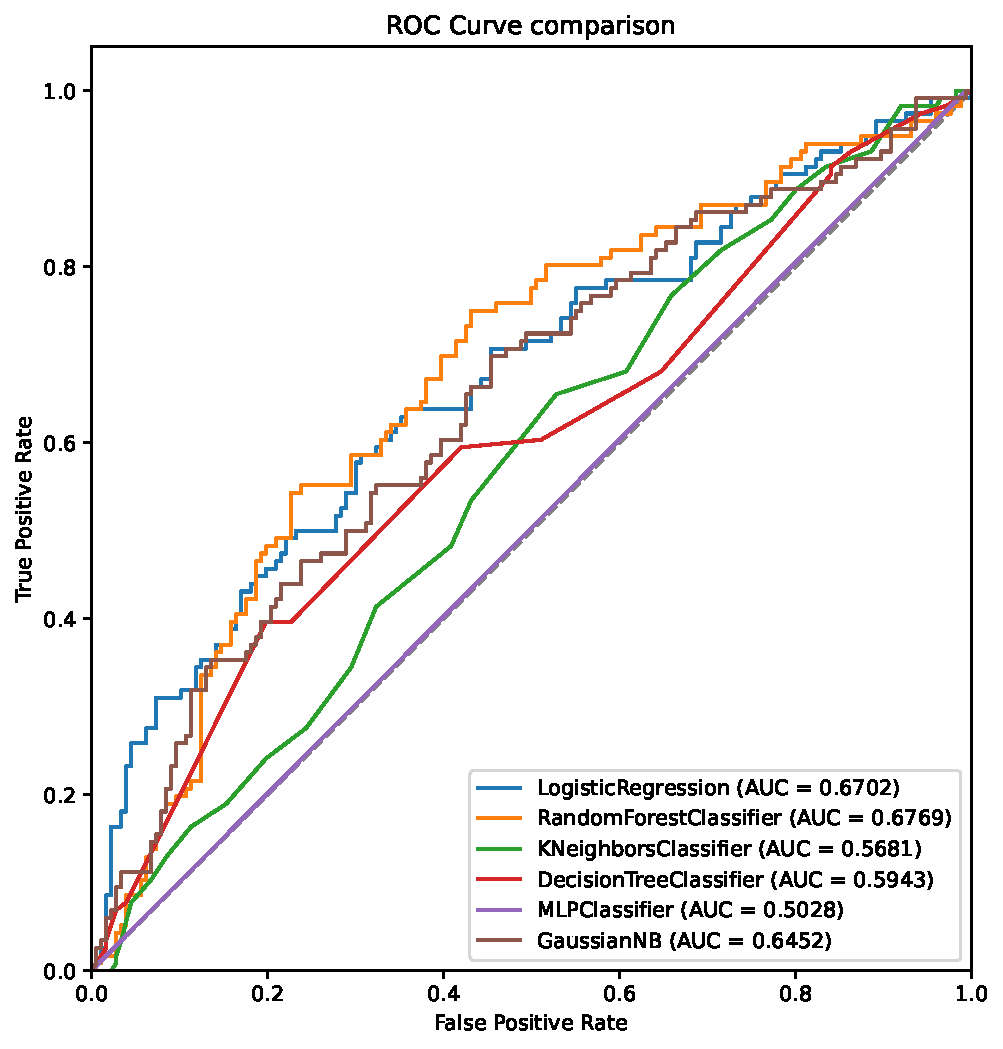
\includegraphics[width=3.1in]{roc_comparison.pdf}
    \caption{\gls{roc} curves comparison.}
    \label{fig:roc-comparison}
\end{figure}

% \subsection{Cross-validation inspection}

% \autoref{fig:crossvalidation_curve} shows the evolution of the CV for the final model.

% \begin{figure}[htpb]
%     \centering
%     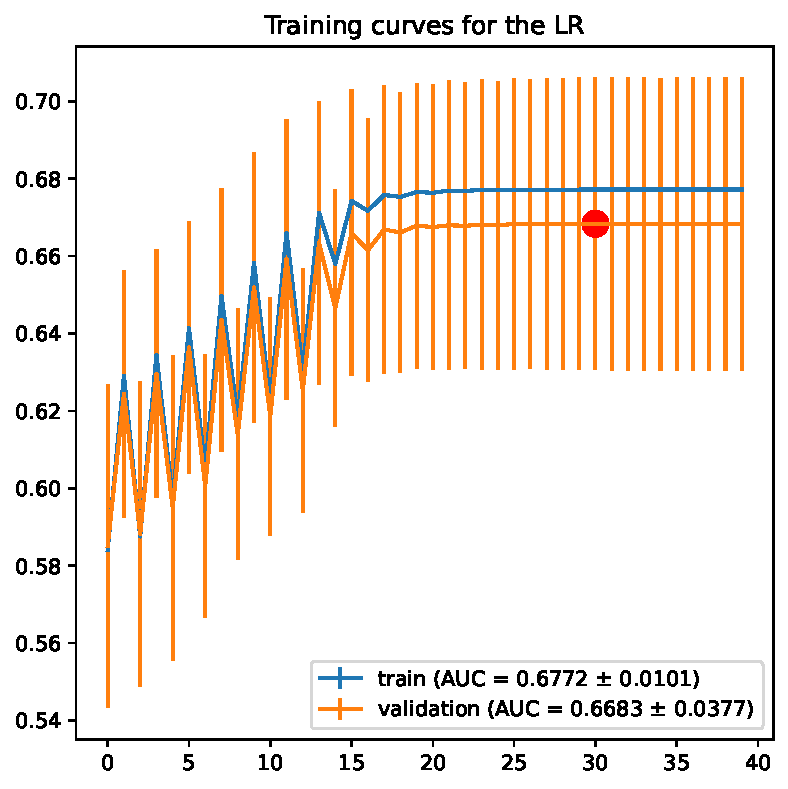
\includegraphics[width=3.1in]{crossvalidation_curve.pdf}
%     \caption{Training evolution.}
%     \label{fig:crossvalidation_curve}
% \end{figure}

\subsection{Model analysis}

Given a vector of variables $\bm{X} = X_1, \dots, X_p$ the \gls{lr} model assumes the following relation between the variables and a prediction score $p(\bm{X})$, where $\beta_0, \beta_1, \dots, \beta_p$ are unknown real coefficients to be numerically estimated.
\begin{align*}
    \operatorname{logit}(p(\bm{X})) &= \log (\operatorname{odds}(p(\bm{X}))) = \log \left( \frac{p(\bm{X})}{1-p(\bm{X})} \right)\\
    & = \beta_0 + \beta_1 X_1 + \cdots + \beta_p X_p
\end{align*}
% Where the odds are therefore
% \begin{align*}
%     \operatorname{odds}p(\bm{X}) = \frac{p(\bm{X})}{1-p(\bm{X})} = e^{\beta_0 + \beta_1 X_1 + \cdots + \beta_p X_p}
% \end{align*}
% One can easily find the inverse relation
% \begin{align*}
%     p(\bm{X}) &= \frac{\exp(\beta_0 + \beta_1 X_1 + \cdots + \beta_p X_p)}{1+\exp(\beta_0 + \beta_1 X_1 + \cdots + \beta_p X_p)}
% \end{align*}
We can give an interpretation to the coefficients: if $\bm{1}_i$ is a vector of all zeros, and with a $1$ in $i$-th position:
\begin{align*}
\operatorname{OR}_i &= \frac{\operatorname{odds}(\bm{X}+\bm{1}_i)}{\operatorname{odds}(\bm{X})} = \frac{\left(\frac{p(\bm{X}+\bm{1}_i)}{1 - p(\bm{X}+\bm{1}_i)}\right)}{\left(\frac{p(\bm{X})}{1 - p(\bm{X})}\right)}\\
&= \frac{e^{\beta_0 + \beta_1 X_1 + \cdots + \beta_i (X_i + 1) + \cdots + \beta_p X_p}}{e^{\beta_0 + \beta_1 X_1 + \cdots + \beta_i X_i + \cdots + \beta_p X_p}} = e^{\beta_i}
\end{align*}
The odds multiply by $e^{\beta_i}$ for every 1-unit increase in $X_i$.
% 
% However, since we scaled the numerical data before fitting the model, the coefficient is intended for a 1-unit increase in the \emph{scaled} variable, but with some manipulation we can retrieve the effect for the original variable.
% \begin{align*}
% \operatorname{OR}_i = \frac{e^{\beta_i (\frac{(X_i+1)-\mu}{\sigma})}}{e^{\beta_i \frac{X_i-\mu}{\sigma}}} = e^{\frac{\beta_i}{\sigma}}
% \end{align*}

%In \autoref{fig:feature-importance-logistic-regression} we have the coefficients of the \gls{lr} for visualizing importance
In \autoref{tab:lr-coeff} we report the $\beta_i$ coefficients for the final model, together with $e^{\beta_i}$.

% \begin{figure}[htpb]
%     \centering
%     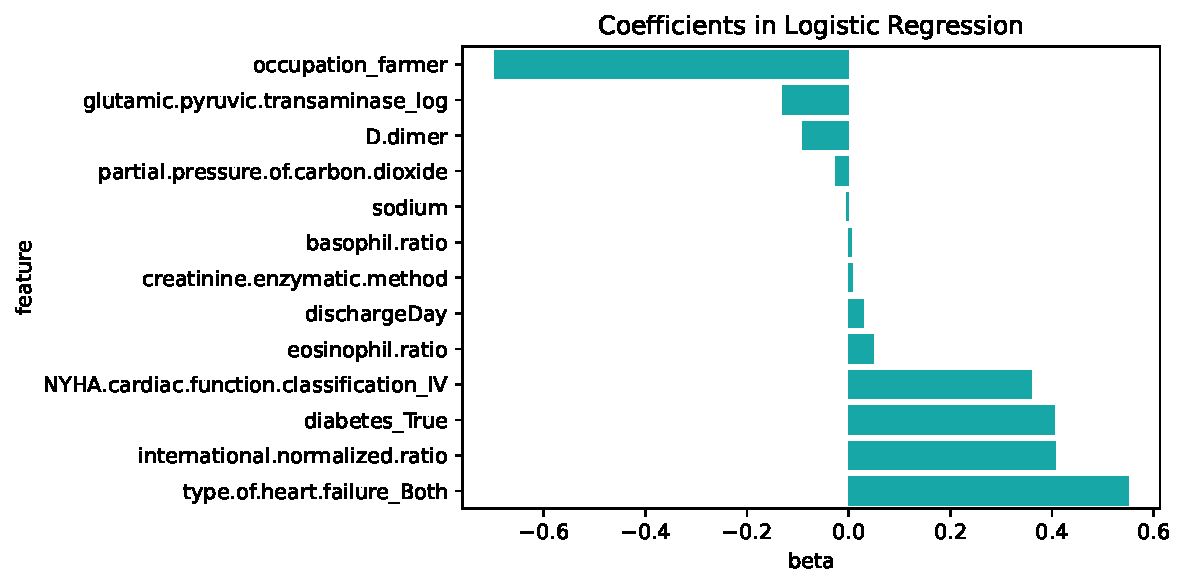
\includegraphics[width=3.1in]{feature_importance_weightsLogisticRegression.pdf}
%     \caption{Coefficients of the \gls{lr}.}
%     \label{fig:feature-importance-logistic-regression}
% \end{figure}

\begin{table}
\centering
\caption{Logistic Regression coefficients.}
\label{tab:lr-coeff}
\begin{tabular}{lrr}
\toprule
                                feature &    beta &  exp\_beta \\
\midrule
                      occupation\_farmer & -0.6973 &    0.4979 \\
      glutamic.pyruvic.transaminase\_log & -0.1305 &    0.8776 \\
                                D.dimer & -0.0911 &    0.9129 \\
     partial.pressure.of.carbon.dioxide & -0.0261 &    0.9743 \\
                                 sodium & -0.0049 &    0.9951 \\
                         basophil.ratio &  0.0055 &    1.0055 \\
            creatinine.enzymatic.method &  0.0066 &    1.0066 \\
                           dischargeDay &  0.0294 &    1.0298 \\
                       eosinophil.ratio &  0.0486 &    1.0498 \\
NYHA.cardiac.function.classification\_IV &  0.3599 &    1.4332 \\
                          diabetes\_True &  0.4049 &    1.4991 \\
         international.normalized.ratio &  0.4074 &    1.5029 \\
             type.of.heart.failure\_Both &  0.5502 &    1.7336 \\
\bottomrule
\end{tabular}
\end{table}


\subsection{Performance evaluation}

The confusion matrix produced by the \gls{lr} obtained with the default threshold of Scikit-learn (0.5) can be seen in \autoref{fig:confusion}, while \autoref{tab:classification-report} contains all the classification metrics.

\begin{figure}[htpb]
\centering
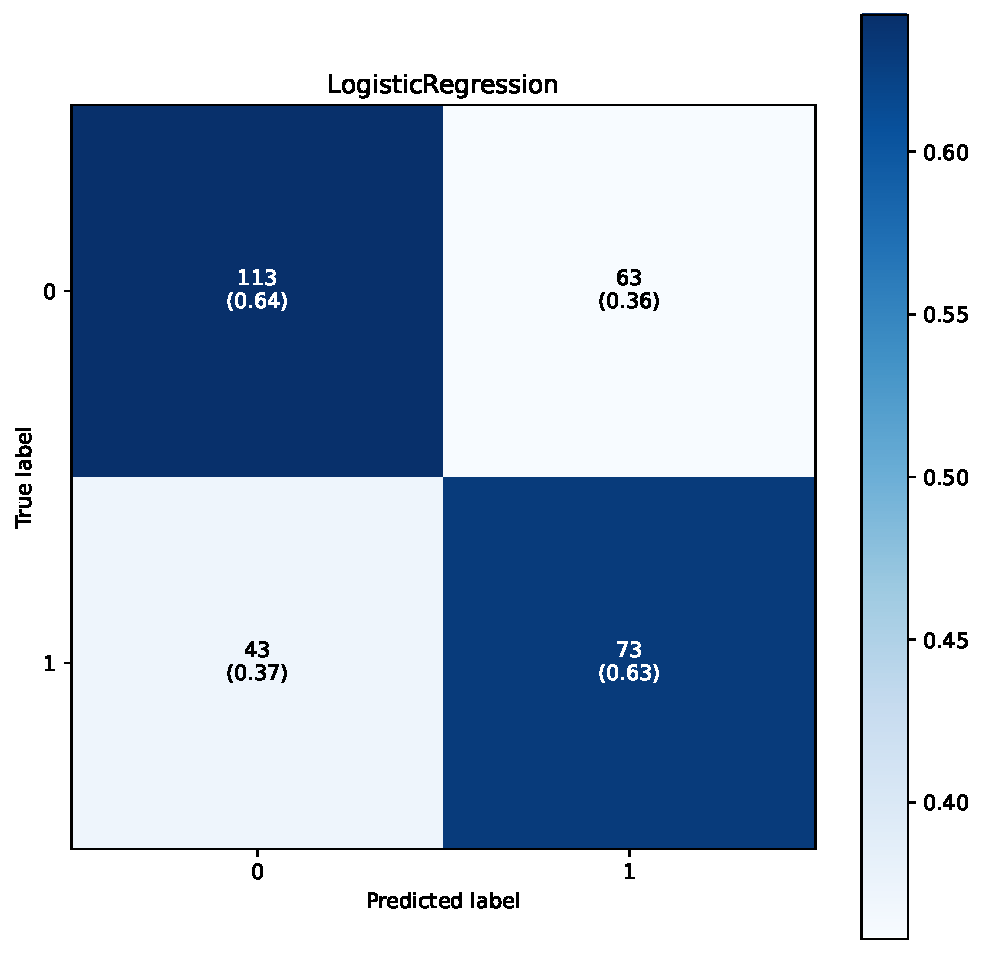
\includegraphics[width=3.1in]{confusion_matrix_LR.pdf}
\caption{Normalized confusion matrix.}
\label{fig:confusion}
\end{figure}

\begin{table}
\centering
\caption{Classification Report.}
\label{tab:classification-report}
\begin{tabular}{rrrr}
\toprule
 precision &  recall &  f1-score &  support \\
\midrule
    0.7244 &  0.6420 &    0.6807 &      176 \\
    0.5368 &  0.6293 &    0.5794 &      116 \\
    0.6306 &  0.6357 &    0.6300 &      292 \\
    0.6498 &  0.6370 &    0.6405 &      292 \\
\bottomrule
\end{tabular}
\end{table}


\subsection{Web App}

Trying to address the needs of clinicians who need user friendly tools to put our statistical results into practice, we developed a web app using the Python library \texttt{streamlit}, to easily input values and get predictions from our final model.

The web app is accessible through the following link:
\url{https://teobucci-slhd-app-3iahgf.streamlit.app/}


%!TEX root = ../report.tex
\section{Discussion and conclusion}

The two most performing models are the \gls{rf} and the \gls{lr} with comparable \gls{auc}, but we chose the latter one for the sake of interpretability. The GaussianNB shows promising performance, while we clearly discard the neural network approach by MLPClassifier.

Looking at the coefficients of the \gls{lr} in \autoref{tab:lr-coeff} there is a strong effect caused by the presence of diabetes, which accounts for an increase in the odds ratio by 1.5; in fact, it is known that diabetes can be responsible for the development of lesions in arteries that are the basis of major cardiovascular diseases.
The presence of a level 4 NYHA accounts for an increase in the odds of 1.43 in favour of a re-admission, an it is indeed symptomatic of severe \gls{hf}, which causes the patient to be bedridden or have serious limitations in their daily activities.
Having suffered from a \gls{hf} of both Left and Right ventricles also accounts for an increase in the odds of 1.7, the strongest of all.

Higher D-dimer and log-transformed glutamic-pyruvic transaminase were associated with lower risk of re-admission.
D-dimer, in healthy conditions, should not be present in the blood, except when a coagulation process is active. High D-dimer values may be a symptom of an increased level of tissue repair following \gls{hf}. However, according to the literature, a high value is not sufficient to confirm this hypothesis.
Strangely, if the patient belonged to the farmer group of occupation, it accounted for a protective odds ratio of about 0.5, but this is likely caused by some external confounder, such as diet and habits of Chinese farmers.

One of the goals was to address drugs importance. None of the 4 categories of drugs identified in \autoref{sec:data-cleaning} made it to the final set of features, so we can't affirm that they are more relevant in predicting re-admission rather than biomarkers.

In fact, according to clinical practice,\footcite{Lonn2000Regular} most patients are treated with both diuretics -- to counteract fluid retention -- and vasodilators -- to prevent the formation of clots -- making these drugs ineffective in predicting readmission to 6 months.
Inhibitors are also poor predictors, as is shown in the literature, because of how variable the effect can be on different patients.
However, among them, the one that proved to be most informative was the \gls{ifhc} that made it to the $S_{\text{reduced}}$ set of features.

%\footcite{Chen2023Predicting}

%admission ward, type of heart failure, NYHA cardiac function classification, diabetes, uric acid, mean hemoglobin volume, basophil count, platelet hematocrit, D dimer, discharge day

%NYHA cardiac function classification, discharge day, uric urea, mean hemoglobin volume, diabetes, and basophil count were associated with higher re-admission risk; when their levels were higher, the patients’ scores were higher. D dimer and platelet hematocrit were associated with lower re-admission. Length of stay in the hospital was also positively associated with the risk of six-month re-admission in HF patients.

\subsection{Comparison with previous models}

%CIT 10.1002/ehf2.12419 developed on datasets with 47 variables and \num{10757} patients in a 30-day prediction obtained an \gls{auc} of 0.501 with RF and 0.628 with MLP. Similar results hold for other studies CIT 
In previous studies\footcite{Sharma2022Predicting} about a 30-day prediction framework, an \gls{auc} of 0.654 was reached using XGBoost, but the authors benefited from having data about prior hospitalization which were ranked as the most important features. Our model was trained without such data and less samples and provided a slightly better performance. The other important variables are aligned with our findings, like sodium and day of discharge.

\subsection{Limitations}

Limitations of this analysis are the difficulty in comparing results with other papers, given that different dataset provide very different variables.

This analysis is also quite biased given that the sample is not representative of the global population, as it comes from a city in China.

Our model also lacked data coming from electrocardiography, which would be well suited for the task.

\subsection{Further development}

We focused on simplicity and interpretability, but for the sake of performance only, one could keep more variables selected by the step-wise methods.

Furthermore, one could explore more advanced classifiers such as XGBoost or AdaBoost, and try an interpretation path through the Shapely value.

It would be interesting to repeat the analysis for the 28-day re-admission and see how the results change; however, this task is not said to be easier given a more prominent imbalance in the data for this class.

\subsection{Recommendations}

Overall we recommend a better management of missing values and a closer look to units of measure. We also iterate about checking the three variables mentioned in \autoref{sec:outlier-analysis}.


% Max 4-5 pages

%\begin{thebibliography}{1}
%\bibitem{IEEEhowto:perez}
%L. Perez and J. Wang}, \emph{The Effectiveness %of Data Augmentation in Image Classification %using Deep Learning} - \relax Stanford %University, 2017.
%\end{thebibliography}

\end{document}